\documentclass[amsmath,secnumarabic,floatfix,amssymb,nofootinbib,nobibnotes,letterpaper,11pt,tightenlines,showkeys]{revtex4}

\usepackage{times}

\usepackage{geometry}
\usepackage{amssymb}
\usepackage{latexsym, amsmath, amscd,amsthm}
\usepackage{graphicx}
\usepackage{array}
\usepackage[percent]{overpic}
%\usepackage{pdfsync}
\usepackage{units}
\usepackage{hyperref}
\PassOptionsToPackage{caption=false}{subfig}
\usepackage[lofdepth]{subfig}

%\usepackage{clrscode}
\usepackage{algorithm}
\usepackage{algpseudocode}

\def\figdir{figs/}
\graphicspath{\figdir}

\newtheorem{theorem}{Theorem}
\newtheorem*{maintheorem}{Main Theorem}
\newtheorem{lemma}[theorem]{Lemma}
\newtheorem{proposition}[theorem]{Proposition}
\newtheorem{corollary}[theorem]{Corollary}

\theoremstyle{definition}
\newtheorem{definition}[theorem]{Definition}
\newtheorem*{example}{Example}
\newtheorem{conjecture}[theorem]{Conjecture}
\newtheorem{remark}[theorem]{Remark}

\def\defn#1{Definition~\ref{def:#1}}
\def\thm#1{Theorem~\ref{thm:#1}}
\def\lem#1{Lemma~\ref{lem:#1}}
\def\figr#1{Figure~\ref{fig:#1}}
\def\prop#1{Proposition~\ref{prop:#1}}
\def\cor#1{Corollary~\ref{cor:#1}}
\def\sect#1{Section~\ref{sect:#1}}
\def\mainthm#1{Main Theorem~\ref{mainthm:#1}}
\def\mainthm#1{Main Theorem~\ref{mainthm:#1}}
\def\rmark#1{Remark~\ref{rmark:#1}}
%\numberwithin{equation}{section}

% make a small change

\newcommand{\abs}[1]{\lvert#1\rvert}
\newcommand{\tvnorm}[1]{\left| #1 \right|_{\operatorname{TV}}}
\newcommand{\R}{\mathbb{R}}
\newcommand{\C}{\mathbb{C}}
\newcommand{\Q}{\mathbb{H}}
\newcommand{\Z}{\mathbb{Z}}
\newcommand{\F}{\mathbb{F}}

\newcommand{\arc}[1]{\gamma_{#1}}
\newcommand{\len}[1]{\ell_{#1}}
\newcommand{\bdry}{\partial}
\newcommand{\bdy}{\bdry}
\newcommand{\isom}{\cong}
\newcommand{\setm}{\smallsetminus}
\newcommand{\eps}{\varepsilon}
\newcommand{\lk}{\textrm{lk}}
\newcommand{\intr}{\textrm{int}} %interior
\newcommand{\half}{\tfrac12}
\newcommand{\arcsec}{\textrm{arcsec}}
\newcommand{\m}{\mathcal}
\renewcommand{\d}{\partial}
\newcommand{\grad}{\nabla}
\newcommand{\PThree}{\ePol_3(n)/\SO(3)}
\newcommand{\EOne}{E_1}
\newcommand{\ETwo}{E_2}
\newcommand{\FOne}{F_1}

\newcommand{\loopinsert}{E_1}
\newcommand{\edgedouble}{E_2}
\newcommand{\cutedgedouble}{E_3}
\newcommand{\pairinsert}{E_4}
\newcommand{\plantri}{\textit{plantri} }
\newcommand{\nauty}{\textit{nauty} }
\newcommand{\saucy}{\textit{saucy} }
\newcommand{\pdcode}{pdcode }
\newcommand{\pdcodes}{pdcodes }

\newcommand{\edges}{\operatorname{edges}}
\newcommand{\head}{\operatorname{head}}
\newcommand{\tail}{\operatorname{tail}}

\graphicspath{{../../figs/}{figs/}}

\newcommand{\eightgraph}{\raisebox{-0.17\baselineskip}{\includegraphics[height=0.81\baselineskip]{eightgraph}}}
\newcommand{\hopfgraph}{\raisebox{-0.17\baselineskip}{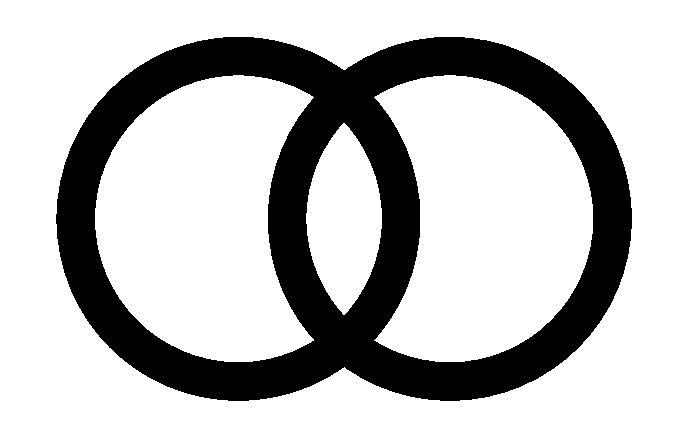
\includegraphics[height=0.81\baselineskip]{hopfgraph.pdf}}}


\bibliographystyle{plain}
%
\def\co{\colon\!}

\setlength{\parskip}{5pt}

\let\mgp=\marginpar \marginparwidth18mm \marginparsep1mm
\def\marginpar#1{\mgp{\raggedright\tiny #1}}
%\def\marginpar#1{}   %Uncomment this to hide all marginpars

\let\lbl=\label
\def\label#1{\lbl{#1}\ifinner\else\marginpar{\ref{#1} #1}\ignorespaces\fi}

\bibliographystyle{plain}

\begin{document}
\title[]{Knot Probabilities in Random Diagrams}
\author{Jason Cantarella, Harrison Chapman}
\altaffiliation{University of Georgia, Mathematics Department, Athens GA}
\noaffiliation
\author{Matt Mastin}
\altaffiliation{Wake Forest University, Mathematics Department, Athens GA}
\noaffiliation

\maketitle

Suppose that one is given an $n$-crossing knot diagram chosen at random from the (finite) set of such diagrams. What is the probability that it is a diagram of the unknot? In this paper, we report on a computer experiment which gives precise answers to this and similar questions for $n \leq 12$ by direct enumeration and classification of knot diagrams. From the point of view of classical knot theory, this is a particularly simple model of random knotting. Part of our interest is to provide data which can be compared to results about more complicated distributions, such as the distribution of knots provided by selecting random closed equilateral $n$-gons, closed lattice walks, or in combinatorial models such as Even-Zohar et.\ al.\'s \emph{Petaluma} model.

\section{Definitions}

We begin with some definitions
\begin{definition}
We define a \emph{link shadow} with $n$ vertices to be an equivalence class of connected $4$-regular embedded planar multigraphs with $n$ vertices up to \emph{shadow isomorphism} which is a graph isomorphism which preserves the counterclockwise order of edges around each vertex.
\end{definition}

Examples of link shadows are shown below
\begin{center}
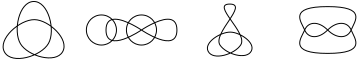
\includegraphics[width=4in]{linkshadow.pdf}
\end{center}
It is well-understood that the equivalence relation preserves the (spherical) embedding of the planar graph; in fact, the left and right-most shadows are actually equivalent under embedded isomorphism-- we have just changed the ``exterior'' face of the projection from the sphere to the plane.

We can partition the edges of a link diagram into \emph{components} by defining two edges to be equivalent if they meet at a vertex at positions which are not cyclicly adjacent. We will call shadows with a single component \emph{knot shadows}. They will be the focus of this paper.

It's standard in knot theory that
\begin{proposition}
The finite set of knot shadows with $n$ vertices is bijective to the finite set of generic immersions of $S^1$ into $S^2$ up to orientation-preserving diffeomorphism of the sphere.
\end{proposition}

We can define a link diagram by
\begin{definition}
A \emph{link diagram} is a link shadow where each component is oriented and each vertex is decorated with over-under information for the edges meeting at the vertex. We call these vertices \emph{crossings}. The equivalence relation for these diagrams is the \emph{diagram automorphism}: a shadow isomorphism which also preserves orientation and over-under information.
\end{definition}
It is clear that there are at most $2^{\text{\# components}} 2^{\text{\# crossings}}$ link diagrams associated to a given link shadow, but that this number may be reduced if there are nontrivial diagram automorphisms.

Various models of random knots have been proposed in the literature. In this paper, we will examine a quite natural one:
\begin{definition}
In the \emph{random diagram model}, a random $n$-crossing knot is selected uniformly from the counting measure on the finite set of one-component $n$-crossing link diagrams.
\end{definition}
We intend to compute knot probabilities directly in the random diagram model for (relatively) small $n$ by direct enumeration of the collection of $n$-crossing random knots. Having the entire collection of diagrams will in addition allow us to study transitions between diagrams, but we will discuss this in future work.

\section{pdcodes and software architecture}

One of us (Mastin) has given a detailed construction of a combinatorial object,  called a PD-code, bijective to the knot diagrams. A PD-code is a set comprised of quadruples, where each entry in a quadruple may be viewed as an edge in a link diagram and each quadruple corresponds to a crossing. PD-codes seem to have been first used by the KnotTheory Mathematica package **cite Knot Atlas** developed by Dror Bar-Natan and his students.

%\begin{center}
%\textbf{Matt summarizes pd codes, defines pd code isomorphism combinatorally, we pick up with the expected algorithm for determining pd isomorphism}
%\end{center}

\begin{definition}\label{def:PD}
Given a link diagram with labeled edges we generate the set of quadruples of the \textbf{PD-code} representing this diagram by the following procedure. For each crossing we include the quadruple of edge labels involved beginning with the incoming under-edge and proceeding around the crossings in the positively oriented direction of $S$ (see Figure~\ref{fig:PD}). We give a positive sign to incoming edges and a negative sign to outgoing edges.

\begin{figure}
\begin{center}
\begin{overpic}[height=4cm]{PD.pdf} %% TODO: Add PD.pdf to SVN
\put(40,35){$1$}
\put(28,15){$2$}
\put(-3,30){$3$}
\put(28,33){$4$}
\put(35,-1){$5$}
\put(16,21){$6$}
\put(55,27){$\{ [+4,-2,-5,+1],[+2,-6,-3,+5],$}
\put(67,21){$[+6,-4,-1,+3]\}$}
\end{overpic}
\end{center}
\caption{\label{fig:PD} A diagram for $3_1$ and its PD-code. The labels are only single integers here as there is only one component. Note that we may omit directional arrows as the orientation can be inferred from the ordering of the edge labels.}
\end{figure}

%\begin{figure}
%\begin{center}
%\begin{overpic}[height=7cm]{PDLink.pdf}
%\put(1,46){$(1,1)$}
%\put(25,37){$(1,2)$}
%\put(39,19){$(1,3)$}
%\put(26,5){$(1,4)$}
%\put(8.5,10){$(1,5)$}
%\put(7,31){$(1,6)$}
%\put(35,43){$(1,7)$}
%\put(41,26){$(1,8)$}
%\put(24,16){$(1,9)$}
%\put(2,15){$(1,10)$}
%\put(22,28){$(2,1)$}
%\put(41,11){$(2,2)$}
%\put(37,2){$(2,3)$}
%\put(11,2){$(2,4)$}
%\put(53,43){$\{[(1,+6),(1,-2),(1,-7),(1,+1)],$}
%\put(55,38){$[(1,+2),(1,-8),(1,-3),(1,+7)],$}
%\put(55,33){$[(2,+1),(1,-9),(2,-2),(1,+8)],$}
%\put(55,28){$[(1,+9),(2,-1),(1,-10),(2,+4)],$}
%\put(55,23){$[(1,+10),(1,-6),(1,-1),(1,+5)],$}
%\put(55,18){$[(2,+2),(1,-4),(2,-3),(1,+3)],$}
%\put(55,13){$[(1,+4),(2,-4),(1,-5),(2,+3)]\}$}
%\end{overpic}
%\end{center}
%\caption{\label{fig:PDLink} A diagram of the link $7_7^2$ and the corresponding PD-code.}
%\end{figure}

%PD-codes that are obtained in the fashion will be called diagramatic PD-codes.

\end{definition}

The details of the bijection between the PD-codes and link diagrams can be found in **cite PD-code Paper**. We will presently include the construction of a cell decomposition of $S^2$ associated with a PD-code as it will play a central roll in our algorithm for enumerating diagrams. The vertices of the cell decomposition will correspond to the quadruples appearing in the PD-code and the edges will be the edges of the diagram. In order to defined the faces we will introduce the \textbf{successor map} which essentially gives the next edge to appear if one were to walk along an edge and turn right a vertex.

\begin{definition}
 If we represent the quadruples in the a PD-code as $[e_i^0,e_i^1,e_i^2,e_i^3]$, then we define the successor map by $s(e_i^j)=-e_i^{j+1 \mod(4)}$.
\end{definition}

We can now define a cell complex associated to a PD-code which recovers the link diagram on $S^2$.

\begin{definition}\label{def:surface}
For each orbit of the successor map $s$ we construct an oriented polygon in the plane with sides given by the labels in each orbit where the labels are assigned clockwise around the polygon. The orientation of an edge agrees with the orientation inherited from the standard orientation of the plane for \emph{negative} labels and disagrees with this orientation for \emph{positive} labels. The orientations of the $2$-cells is inherited from the standard orientation on the plane. The orientations of the edges is induced by the orientation of the $2$-cells. This construction gives the \textbf{associated cell complex} to a given PD-code.
\end{definition}

This construction gives a collection of oriented polygons in the plane whose edges are labeled by the edge labels of the given link diagram. If these polygons are glued according to the edge labels and orientations then the link diagram is reconstructed as the $1$-skeleton of the resulting cell complex. The details of this construction can be found in **cite PD-code Paper**.

\begin{definition}\label{def:PDIsom}
	Given two PD-codes we say that a bijection between the edge labels is a \textbf{PD-code isomorphism} if it induces an isomorphism on the associated cell complexes.
\end{definition}

It is clear that a lot of data about a \pdcode is preserved by isomorphism: for instance, the number of crossings, edges, faces, and the numbers of edges around faces. We can use this information to rule out isomorphisms using a hashing scheme.

\begin{definition}
Suppose the \pdcode $P$ has $V$ crossings, $E$ edges, $F$ faces, and $C$ components. We assume that the faces are denoted $f_1, \dots, f_F$ and the components are denoted $c_1, \dots, c_C$. Further, let $\edges(x)$ give the number of edges on a face or component. Then the \emph{hash} of $P$ is given by the tuple
\begin{equation*}
\mathcal{H}(P) = (V,E,F,C,\{ \edges(f_1), \dots, \edges(f_F) \},
 \{ \edges(c_1), \dots, \edges(c_C) \}).
\end{equation*}
The last two are unordered sets of integers.
\end{definition}

It is clear that
\begin{lemma}
If two \pdcodes $P_1$ and $P_2$ are isomorphic, then $\mathcal{H}(P_1) = \mathcal{H}(P_2)$.
\end{lemma}

\begin{proof}
The numbers $V$, $E$, $F$, and $C$ are clearly preserved by isomorphism. The indices of edges and faces may be permuted by an isomorphism, but the number of edges on each can't change. Thus the \emph{unordered sets} of edge counts for faces and component remain the same as well.
\end{proof}

We can now build up an isomorphism between pdcodes by a series of definitions:

\begin{definition}
Suppose we have two pdcodes $P$ and $P'$ with the same hash.
\begin{itemize}
\item A bijection $\gamma: \{c_1,\dots,c_C\} \rightarrow \{c'_1,\dots,c'_C\}$ between the components of $P$ and the components of $P'$ is called \emph{component-length preserving} if $\# \edges(c_i) = \# \edges(\gamma(c_i))$ for all $i$.
\item Given such a component-length preserving bijection $\gamma$, a bijection $\epsilon : \{e_1,\dots,e_E\} \rightarrow \{e'_1,\dots,e'_E\}$ between the edges of $P$ and the edges of $P'$ is called \emph{component-preserving} and \emph{compatible with $\gamma$} if $\epsilon$ maps the edges of each $c_i$ to the edges of $\gamma(c_i)$ by an element of the dihedral group $D_{\edges(c_i)}$. That is, the edges of $c_i$ are mapped in cyclic (or reverse-cyclic) order to the corresponding edges of $\gamma(c_i)$.
\item Given a component-preserving bijection $\epsilon : \{e_1,\dots,e_E\} \rightarrow \{e'_1,\dots,e'_E\}$ between the edges of $P$ and the edges of $P'$, we say that a bijection $\nu : \{v_1, \dots, v_V\} \rightarrow \{v'_1,\dots,v'_V\}$ between the vertices of $P$ and the vertices of $P'$ is \emph{compatible with $\epsilon$} if
\begin{equation*}
\nu(\head(e_i)) = \head(\epsilon(e_i)) \quad \text{ and } \quad \nu(\tail(e_i)) = \tail(\epsilon(e_i)
\end{equation*}
when $e_i$ is part of a component mapped by an orientation-preserving element of the dihedral group, and
\begin{equation*}
\nu(\head(e_i)) = \tail(\epsilon(e_i)) \quad \text{ and } \quad \nu(\tail(e_i)) = \head(\epsilon(e_i)
\end{equation*}
when $e_i$ is part of a component mapped by an orientation-reversing element of the dihedral group.
\item Given $\gamma$, $\epsilon$, and $\nu$ that obey all the above conditions, we say that they are:
\begin{itemize}
 \item \emph{globally orientation-preserving} if the set of edges $e_i, e_j, e_k, e_l$ incident to each vertex $v$ of $P$ (in counterclockwise cyclic order) is mapped to the set of edges $\epsilon(e_i), \epsilon(e_j), \epsilon(e_k), \epsilon(e_l)$ incident to $\nu(v)$ in counterclockwise cyclic order.
 \item \emph{globally orientation reversing} if the $\epsilon(e_i), \epsilon(e_j), \epsilon(e_k), \epsilon(e_l)$ are incident to $\nu(v)$ but in clockwise cyclic order (for each $v$),
 \item otherwise, the triple is \emph{inconsistent}.
\end{itemize}
\end{itemize}
\end{definition}

We then have
\begin{proposition}
Given a pair of pdcodes $P$ and $P'$ with the same hash, each isomorphism of $P$ to $P'$ is given by a set of bijections $\gamma$ between their components, $\epsilon$ between their edges, and $\nu$ between their vertices where
\begin{itemize}
\item $\gamma$ is component-length preserving,
\item $\epsilon$ is component-preserving and compatible with $\gamma$,
\item $\nu$ is compatible with $\epsilon$
\end{itemize}
and the triple is globally orientation preserving or reversing (not inconsistent).
\end{proposition}

\begin{proof}
Basically, this is the definition of pd isomorphic.
\end{proof}

A few other observations are helpful:
\begin{lemma}
If $\mathcal{H}(P) = \mathcal{H}(P')$ for pdcodes $P$ and $P'$, there is at least one component-length preserving $\gamma : \{c_1,\dots,c_C\} \rightarrow \{c'_1,\dots,c'_C\}$. All component-length preserving $\gamma$ can be generated by iterating over a product of permutation groups.
\end{lemma}

\begin{proof}
We can partition the components of $P$ (and $P'$) into subsets by component length. Since the hashes $\mathcal{H}(P)$ and $\mathcal{H}(P')$ match, these partitions correspond for $P$ and $P'$. The component-length preserving $\gamma$ are exactly those bijections which respect this partition: we can construct all such $\gamma$ by taking a product of permutation groups whose orders are the size of the subsets. At worst, all subsets have size 1 and there is a single such $\gamma$.
\end{proof}

\begin{lemma}
Given a component-length preserving $\gamma$ and component-preserving and compatible $\epsilon$, and a set of orientations for the components of $P$, there is at most one $\nu : \{v_1, \dots, v_V\} \rightarrow \{v'_1,\dots,v'_V\}$ which is compatible with $\epsilon$ and consistently oriented on components and we can construct $\nu$ as below.
\end{lemma}

\begin{proof}
Each vertex $v$ of $P$ is incident to four edges $e_i, e_j, e_k, e_l$. Without loss of generality, let's assume that $v = \tail(e_i)$, $\tail(e_j)$, $\head(e_k)$ and $\head(e_l)$. Then if $\nu$ is compatible with $\epsilon$, we must have
\begin{equation*}
\nu(v) = \tail(\epsilon(e_i)) = \tail(\epsilon(e_j)) = \head(\epsilon(e_k)) = \head(\epsilon(e_l)).
\end{equation*}
If the four terms on the right are equal, this uniquely defines $\nu(v)$. If not, there is no compatible $\nu$.
\end{proof}

We can now find all isomorphisms between two pdcodes computationally by a simple brute-force strategy:

\begin{algorithm}
\begin{algorithmic}[1]
\Procedure{BuildIsomorphisms}{$P$,$P'$}
\Comment{Build isomorphisms between pdcodes $P$ and $P'$}

\If {the hashes $\mathcal{H}(P)$ and $\mathcal{H}(P')$ are different}
	\State $P$ and $P'$ are not isomorphic. Return $\emptyset$.
\EndIf

\ForAll{component-length preserving $\gamma: \{c_1,\dots, c_C\} \rightarrow \{c'_1, \dots, c'_C\}$}
	\ForAll{compatible and component-preserving $\epsilon$}
		\If{a compatible $\nu$ exists}
		\If{$\nu$ is globally orientation preserving or reversing}
			\State $\epsilon$, $\nu$ define an isomorphism $P \rightarrow P'$
		\EndIf
		\EndIf
	\EndFor
\EndFor
\EndProcedure
\end{algorithmic}
\end{algorithm}

It should be immediately clear that there are smarter ways to organize this computation: for instance, we could build only part of $\gamma$ and $\epsilon$ before we start checking the consistency conditions for the existence of a compatible $\nu$. Or we could map faces to faces by elements of the dihedral group on the grounds that faces are smaller than components. Or we could try for a more complicated hashing scheme which took into account the adjacency relations between faces. These sorts of ideas are implemented with great insight and care in graph isomorphism packages like \nauty and \emph{saucy}. However, making these types of changes makes the code more intricate and difficult to debug: in this project, our overall strategy is to use simple, straightforward algorithms in the hopes of minimizing the chance of errors.

\section{Constructing the database of diagrams}

Our first goal is to enumerate the link shadows-- that is, the connected 4-regular embedded planar (multi)graphs-- computationally. Since this is the heart of our work, we describe two independent algorithms for the enumeration. One is quite simple while the other is much more complex. We implemented, tested, and ran both of them independently to generate the database of diagrams, verifying that the results of the computations were the same.

\subsection{Dual quadrangulations and connect sums}

Brinkmann et.\ al.~\cite{Brinkmann:2007up} provided an algorithm to enumerate all of the simple embedded planar quadrangulations of $S^2$, up to embedded isomorphism. A quadrangulation is a planar graph where each face has four edges, as in the pictures below.
\begin{center}
\includegraphics[height=1.25in]{quadrangulations-example}
\end{center}
The dual graph to a quadrangulation is a connected 4-regular embedded planar multigraph, as shown below left. However, if the quadrangulation is simple, the dual graph is what we will call a \emph{prime} diagram: it cannot be decomposed by embedded circles which intersect the diagram in only two edges. We will call diagrams with such a system of decomposing circles \emph{composite}; an example of a non-simple quadrangulation and its (composite) dual graph is shown below right.
\begin{center}
\hphantom{.}
\hfill
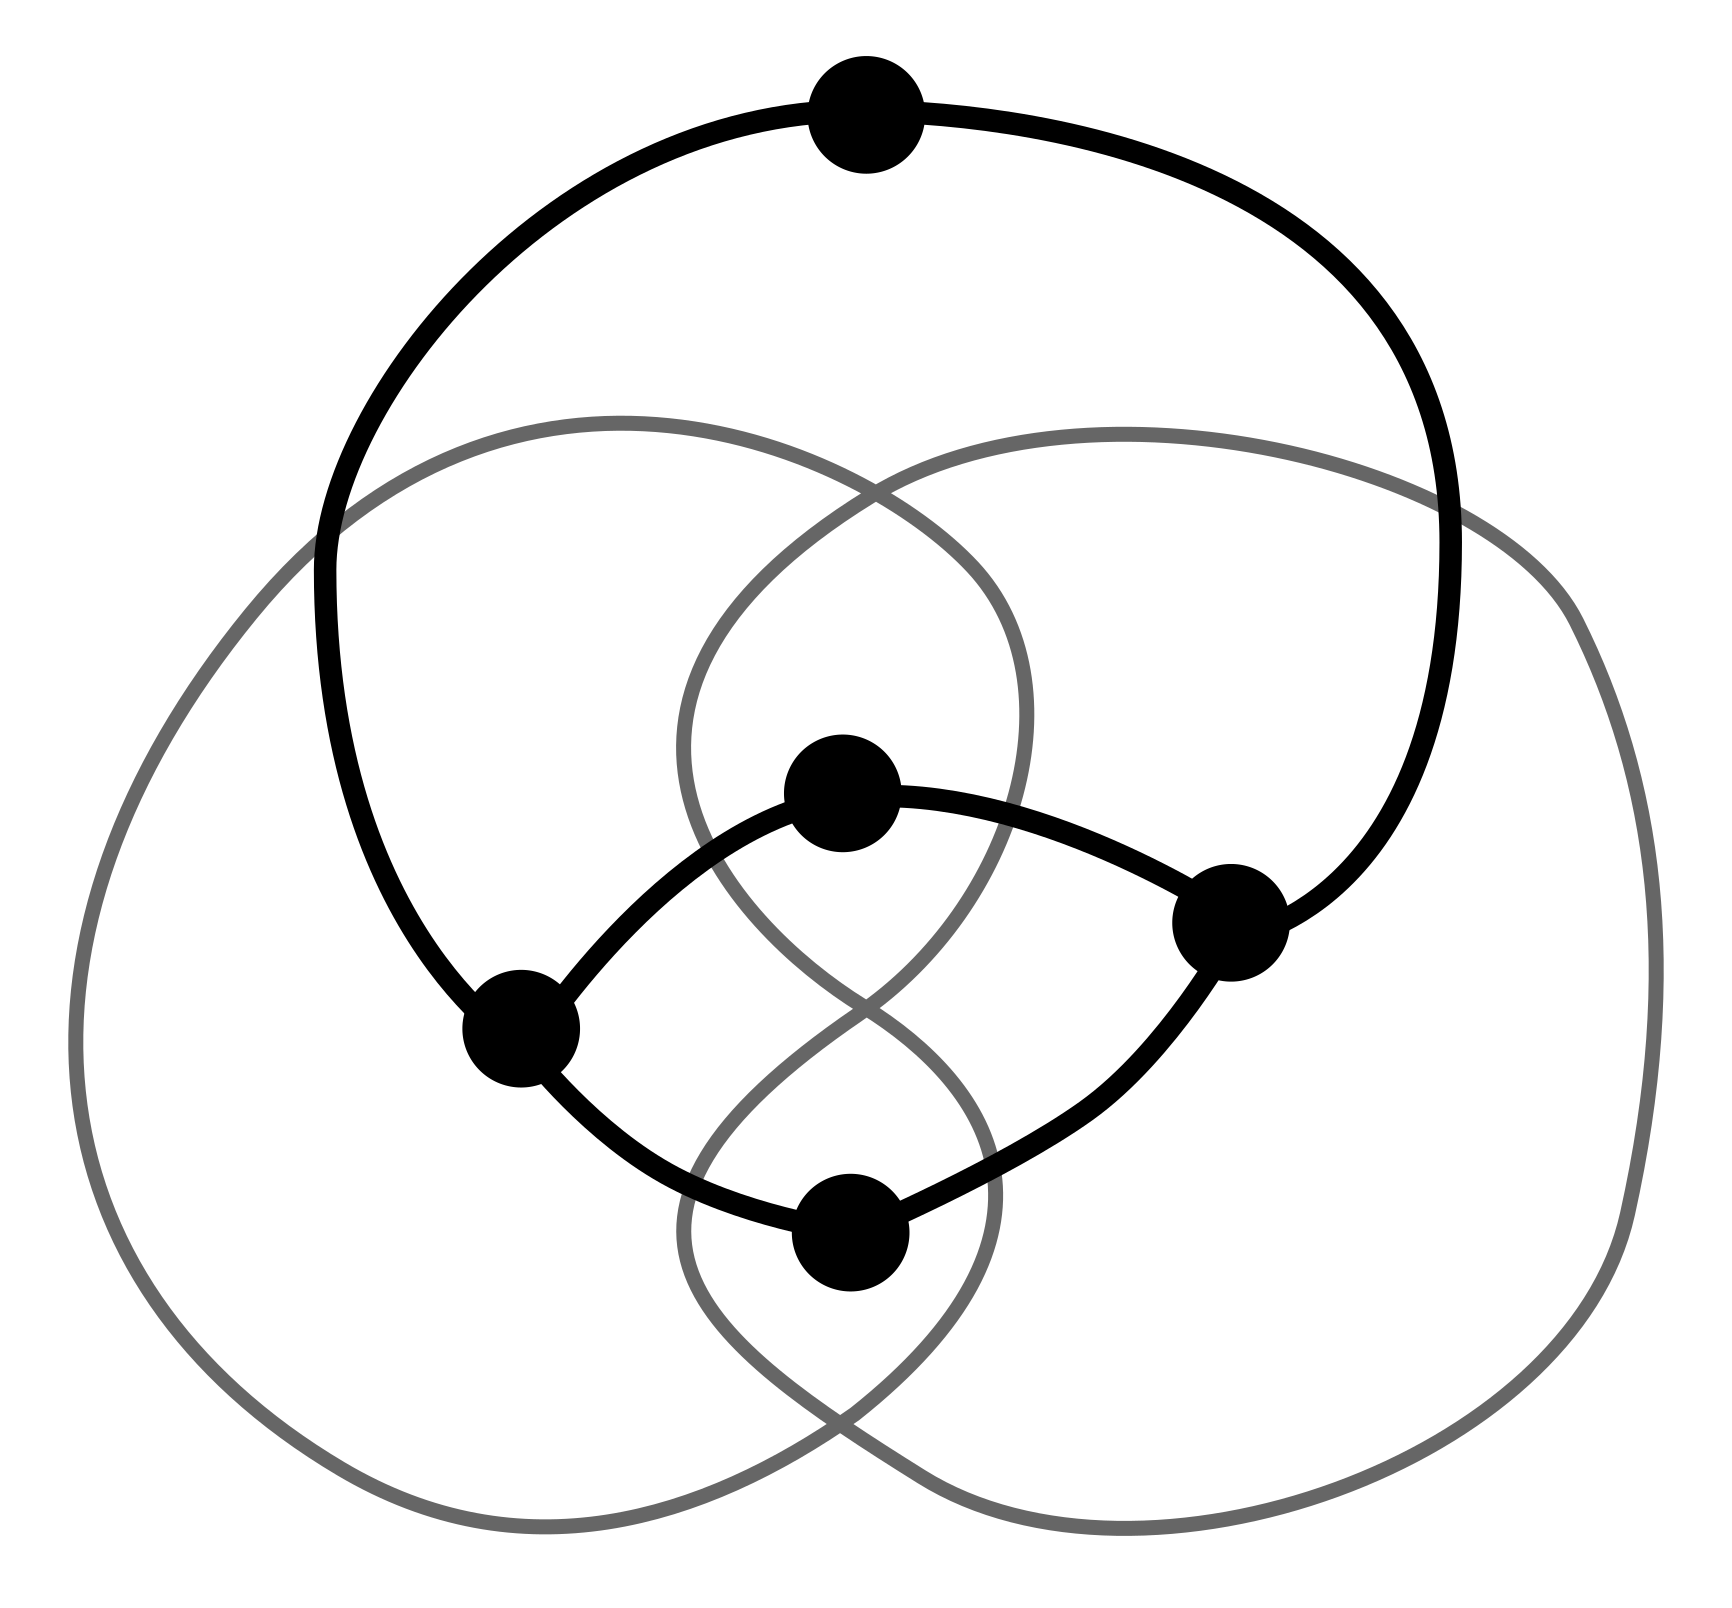
\includegraphics[height=1.25in]{quadrangulation} \hfill
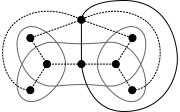
\includegraphics[height=1.25in]{non-simple-quadrangulation}
\hfill
\hphantom{.}
\end{center}
The \plantri software of Brinkmann and McKay~\cite{Brinkmann:2007up,McKay:1998wa} can be used to generate the dual graphs of the planar simple quadrangulations of given number of vertices. Since an easy Euler characteristic argument shows that the number of vertices in the dual graph of a quadrangulation is 2 less than the number of vertices in the quadrangulation, we can use this to enumerate the connected 4-regular embedded planar multigraphs which are prime.

To enumerate all diagrams, we recall (as is standard in knot theory) that every composite diagram is uniquely expressed as a collection of prime diagrams joined along pairs of edges by the connect sum operation. Of course, this regularly generates isomorphic diagrams when the prime diagrams have a nontrivial automorphism group. It would be interesting and fun to predict when this happens and arrange to avoid generating duplicate diagrams by tracking edge orbits under the automorphism group of each diagram. However, in keeping with our strategy of simple, robust code, we simply construct all connect sums iteratively and check for isomorphisms with existing pdcodes using the hashing/brute force strategy for isomorphism checking detailed above. The process is shown below

\begin{center}
\includegraphics[width=3in]{composite-workflow}
\end{center}

where the arrows indicate ``all possible connect sums (and entry into the database with isomorphic copies of an existing diagram rejected)'' or simply ``entry into the database with isomorphic copies rejected''.

\subsection{Expansions of embedded planar simple graphs}

Our next strategy will be much more complicated (and somewhat slower to run), but it serves as crucial check on the previous computation. The basic idea is to define a smaller class of graphs so that the graphs we are interested in can be obtained from the base class of graphs by various expansion moves. Lehel~\cite{JGT:JGT3190050412} gave a strategy for generating all 4-regular graphs in this way from the octahedral graph. Instead of using Lehel's strategy directly, we build on the method of Brinkmann and McKay~\cite{Brinkmann:2007up,McKay:1998wa} for enumerating isomorph-free embedded planar graphs; we extend their work here to generate the class of graphs that we're interested in.

We now define four expansion moves of embedded planar graphs with vertex degree $\leq 4$ which generate new embedded planar graphs of vertex degree $\leq 4$ with the same number of vertices, but additional edges:
\begin{definition}
The four expansion operations that we will use are the following:
\begin{itemize}
\item $\loopinsert$ Loop insertion adds a loop edge to a vertex of degree 1 or 2, as below. (Note: Loop insertion can be performed on each side of a vertex of degree 2).\\
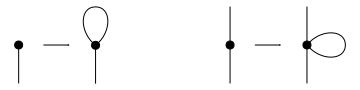
\includegraphics[width=4in]{loop-addition.png}
\item $\edgedouble$ reversing edge doubling duplicates an existing edge joining vertices of degree $< 4$ so as to create a new bigon face. Note that the (counterclockwise) order of the two vertices is reversed on the two vertices.\\
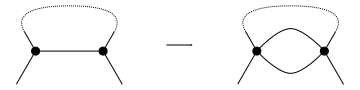
\includegraphics[width=4in]{edge-duplication-non-cut.png}
\item $\cutedgedouble$ preserving doubling also duplicates an existing edge joining vertices of degree $<4$, but
keeps the counterclockwise order of the edges the same on each at each of the two vertices. This sort of doubling is only available if the original edge is a cut edge of the graph.\\
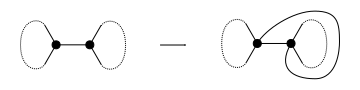
\includegraphics[width=4in]{edge-duplication-cut}
\item $\pairinsert$ pair insertion adds a pair of edges simultaneously, joining two vertices of degree 2 which are both on two faces of the embedding, as below.\\
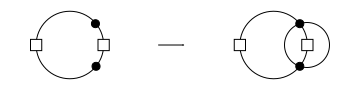
\includegraphics[width=4in]{pair-insertion}
\end{itemize}
\end{definition}

We can now show

\begin{proposition}
Every connected $4$-regular embedded planar (multi)graph $G$ can be obtained from a connected, embedded planar simple graph of vertex degree $\leq 4$ $G_0$ by a series of $\loopinsert$, $\edgedouble$, $\cutedgedouble$, and $\pairinsert$ expansions.

Equivalently, any connected $4$-regular embedded planar (multi)graph $G$ can be reduced to a connected embedded planar simple graph $G_0$ of vertex degree $\leq 4$ by a series of $\loopinsert$, $\edgedouble$, $\cutedgedouble$, and $\pairinsert$ reductions. The embedded isomorphism type of $G_0$ is determined by the  embedded isomorphism type of $G$ (the order in which the reductions are performed doesn't matter).
\label{prop:reduce}
\end{proposition}

An illustration of the process we describe is
\begin{center}
\includegraphics[width=4in]{expansion-from-simple-graph}
\end{center}

\begin{proof}
We will prove the second statement, reducing in stages from some $G_n = G$ to $G_0$ by performing one reduction at each step. The number of steps we can perform is clearly finite, since each reduces the number of edges by at least one. So suppose we are at stage $G_i$. If there are no loop or multiple edges, we're done, and this is the simple graph $G_0$.

If there is a loop edge, we can remove it with a $\loopinsert$ move.

If there is a multiple edge, we must consider several cases. We can think of each vertex of $G_i$ as retaining a list of 4 connection points, ordered counterclockwise, from the initial embedding of $G$. Since we have performed some reductions already, some of these may be empty, but at least two are filled at each end of the multiple edge. Pick one vertex of the multiple edge and call it $v$ and the other vertex $w$.

If the edge multiplicity is four, $G$ is \hopfgraph. This is obtained from the graph with one edge and two vertices by three $\edgedouble$ moves.

If the edge multiplicity is three or two, there is at least one connection point on $v$ which is not occupied by a copy of the multiple edge followed immediately by a connection point which is occupied by a copy $e$ of the multiple edge. Without loss of generality, we'll call $e$ the \emph{base copy} of the multiple edge, and its connection point to at $v$ position $0$ around $v$. The remaining connection points will be numbered $1$, $2$, and $3$. By construction, the edge joined to $v$ at position $3$ (if any) is not connected to $w$. We can label the other end of the base copy $e$ position $a$ on the second vertex $w$, and label the other positions $b$, $c$, and $d$, again counterclockwise.

If the edge multiplicity is three, only one of these positions is unoccupied by a copy of the multiple edge. Looking at the three cases (below), we can see that by parity, it must be position $b$, and the pair of copies $0a$ and $2c$ of the multiple edge can be removed by a $\pairinsert$ operation.
\begin{center}
\includegraphics[width=4in]{multiplicity-three}\\
By parity, because we came from a 4-regular embedded planar graph only the leftmost case can occur at any stage in the reduction process.
\end{center}
We have now disposed of the case where edge multiplicity is three.

If edge multiplicity is two, there is one edge unaccounted for, which joins either position $1$ or $2$ on vertex $v$ to position $b$, $c$, or $d$ on vertex $w$. Therefore, there are six cases to address. We consider them in order, starting with the $1x$ configurations.
\begin{itemize}
\item
\begin{tabular}{m{1in}m{3in}m{1in}}
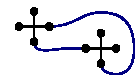
\includegraphics[width=0.9in]{1-b-configuration.pdf}
&
In the $1b$ configuration, the multiple edge forms a 2-cycle dividing the portion of the graph $G$ connected to $cd$ from the portion connected to $23$. Deleting $1b$ requires a $\cutedgedouble$ move, and the remaining base edge is a cut edge of all further-reduced $G_i$, as shown at right.
&
\includegraphics[width=0.9in]{1-b-target}
\end{tabular}
\item
\begin{tabular}{m{1in}m{3in}}
\includegraphics[width=.9in]{1-c-configuration.pdf}
&
The $1c$ configuration is forbidden by parity.
\end{tabular}
\item
\begin{tabular}{m{1in}m{3in}m{1in}}
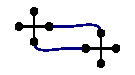
\includegraphics[width=0.9in]{1-d-configuration.pdf}
&
In the $1d$ configuration, the multiple edge forms a bigon face. Deleting $1d$ uses an $\edgedouble$ reduction, and yields the configuration at right. The remaining base edge may or may not be a cut edge of the further $G_i$.
&
\includegraphics[width=0.9in]{1-d-target}
\end{tabular}
\end{itemize}
One might think that the $2-$ configurations are simply rearrangements of those above, but this is not true. A genuinely new case arises for $2c$.
\begin{itemize}
\item
\begin{tabular}{m{1in}m{3in}}
\includegraphics[width=0.9in]{2-b-configuration.pdf}
&
The $2b$ configuration is forbidden by parity.
\end{tabular}
\item
\begin{tabular}{m{1in}m{3in}m{1in}}
\includegraphics[width=.9in]{2-c-configuration.pdf}
&
In the $2c$ configuration, by parity, the graph $G$ must have connected $1$ and $d$ and also $3$ and $b$. None of our moves change the connectivity of the graph (because we never delete all copies of a multiple edge), so the current graph $G_i$ still joins these pairs of connection points. This means that we are in position for an $\pairinsert$ pair reduction, resulting in the graph at right.
&
\includegraphics[width=1in]{2-c-target}
\end{tabular}
\item
\begin{tabular}{m{1in}m{3in}}
\includegraphics[width=0.9in]{2-d-configuration.pdf}
&
The $2d$ configuration is forbidden by parity.
\end{tabular}
\end{itemize}
Along the way, our analysis has been entirely local: we need only consider a single vertex to decide whether we can apply an $\loopinsert$ reduction and a pair of vertices to decide on $\edgedouble$, $\cutedgedouble$, and $\pairinsert$ operations. To show that order of operations doesn't matter, we need to show that whether or not we can apply these operations does not depend on which reductions have already been performed. First, we note that since we never remove all copies of multiple edge, we never change the connectivity of the graph during the reduction process.

The three copies of a multiplicity three edge must bound two bigons, and this does not change as we reduce other edges. Therefore, the $\pairinsert$ move is always available for all multiplicity three edges.

Whether a multiplicity two edge is eligible for an $\edgedouble$ move depends only on the positions of the ends of the multiple copies on their vertices, which doesn't change as we reduce. Therefore, this operation can always be performed (or is always forbidden), regardless of which reductions have already been performed.

Whether a multiplicity two edge is eligible for a $\cutedgedouble$ or $\pairinsert$ operation depends not only on the positions of ends of edges on their vertices, but also on the connectivity of the (reduced) graph. However, as we noted above, the connectivity of the graph doesn't change as we perform reductions.

It is clear that the isomorphism type of $G_0$ does not depend on the order of reduction-- after all, in the end we are simply reducing the multiplicity of multiple edges of the edge.

It takes only a moment longer to realize that the embedding of $G_0$ is determined as well-- this embedding is determined by the cyclic order of (surviving) edges around their vertices. We will have deleted some edges from many of these vertices by the time we reach $G_0$, potentially leaving many empty connections. However, the cyclic order of the surviving edges won't be affected by the order in which these connections were emptied.

One might worry that the choice of \emph{which}\footnote{Remember that the choice of ``base edge'' was arbitrary.} copy of an edge of multiplicity two to delete could affect the embedded isomorphism type after an $\edgedouble$ or $\cutedgedouble$ reduction, but it's easy to check that the two possible reduced configurations are (embedded) graph isomorphic by looking at the pictures above. Formally, the point is that the two copies of the edge are adjacent in the cyclic ordering of edges at each vertex, so the surviving copy is always in the same cyclic position relative to surviving edges incident to the vertex.
\end{proof}

We can use this theorem to come up with a strategy for generating diagrams. Basically, we will start by enumerating embedded planar simple graphs of vertex degree $\leq 4$ using \plantri, then expand them to $4$-regular embedded planar graphs using the moves above. Afterwards, we will see that we can generate embedded isomorphic graphs with different expansion sequences, so we will have to filter the graphs into isomorphism classes. We start with two lemmas:

\begin{lemma}
If the embedded planar graph of vertex degree $\leq 4$ $G_0$ is obtained from a $4$-regular embedded planar multigraph $G$ by the reduction process of Proposition~\ref{prop:reduce} then either every vertex of degree one in $G_0$ has exactly one loop edge in $G$ and one multiedge of multiplicity two obtained by $\edgedouble$ or $\cutedgedouble$ or the graph is \hopfgraph.
\label{lem:degreeone}
\end{lemma}

\begin{proof}
If we expand $G_0$ to $G$ using the four moves, three empty connections on the vertex must be filled during the process. If they are filled by redoubling the existing edge, then the degree of the vertex at the other end of the edge was also one, and we get \hopfgraph. Otherwise, we must fill two by adding a loop edge, and the other by doubling the existing edge.
\end{proof}

\begin{lemma}
Two pairs of vertices $ab$ and $cd$ on the unit circle may be joined by nonintersecting chords inside the circle if and only if the pairs are unlinked on the circle. That is, if $ab$ and $cd$ are adjacent in the cyclic ordering of the four vertices, as opposed to an order such as $acbd$ or $adbc$ where the pairs alternate.
\end{lemma}

We can now design an algorithm to produce all possible expansions of $G_0$, a given connected embedded planar simple graph of vertex degree $\leq 4$ as an integer constraint satisfaction problem. By Lemma~\ref{lem:degreeone}, we must add a loop to each vertex of degree one in $G_0$ eventually. We can save time by doing so at the start of the computation. We will therefore assume that loops have been added to create a \emph{prepared} graph $G_1$, and each vertex has degree $2$, $3$, or $4$.

We will now define four classes of variables:
\begin{itemize}
\item $l_{i}$ for every vertex $v_i$ of degree $2$
\item $d_{i,j}$ for every non-cut edge $e_{ij}$ in the graph joining vertices of degree $<4$.
\item $c_{i,j}$ for every cut edge $e_{ij}$ joining vertices of degree $<4$.
\item $p_{i,j}$ for every pair of vertices $v_{i}$, $v_j$ which both have degree 2 and are both on two different faces of the embedding
\end{itemize}
We take the subscripts to be unordered. That is, $d_{4,17}$ and $d_{17,4}$ are the same variable, since the edges $e_{4,17}$ and $e_{17,4}$ are the same edge.

These variables will all be valued in $0-1$, and represent the absence or presence of $\loopinsert$ loop edges, $\edgedouble$ or $\cutedgedouble$ doubles of existing edges and $\pairinsert$ insertions of new pairs of edges.
We can now define two sets of equations relating these variables.

\begin{definition}
We define the \emph{vertex degree equations} for a prepared graph $G_1$ to be the collection of equations indexed by the vertices of $G_1$ given below. For each vertex index $i$ of degree $\delta(i)$ in $G_1$
\begin{equation*}
\delta(i) + 2 l_i + \sum_j d_{i,j} + \sum_j c_{i,j} + 2 \sum_j p_{i,j} = 4
\end{equation*}
where the sums are taken over all $j$ for which the appropriate variables exist. These equations express the fact that in a complete expansion, the vertex degrees must all be four.
\end{definition}

The pair variables $p_{i,j}$ satisfy an additional set of equations:
\begin{definition}
For each $p_{i,j}$ and $p_{k,l}$ so that the vertices $v_i, v_j, v_k$ and $v_l$ are on the same pairs of faces, and so that the vertices are in the (cyclic) order $v_i, v_k, v_j, v_l$ or $v_i, v_l, v_j, v_k$ we have an additional \emph{linking equation}
\begin{equation*}
p_{i,j} + p_{k,l} \leq 1
\end{equation*}
\end{definition}

These equations express the fact that the edges corresponding to a linked pair of endpoints along a face must intersect inside the face. Therefore, if two pair variables are linked, at most one of them can take the value $1$. For instance, in the situation below where there are four vertices of degree two along a pair of faces, we have six pair variables, two of which obey an additional linking equation.
\begin{center}
\includegraphics[height=1.5in]{linked-ghost-pairs}
\end{center}
We note that in the end, at most two of the pair variables above can have value $1$, but that a number of combinations are ruled out by vertex degree equations instead of linking equations.

We have defined everything so that

\begin{proposition}
Every assignment of $\{0,1\}$ to the variables $l_i$, $d_{i,j}$, $c_{i,j}$, and $p_{i,j}$ which obeys the vertex degree equations and linking equations corresponds to an expansion of the connected planar graph $G_1$ with vertex degrees $2$, $3$, and $4$ and loop edges only to a collection of embeddings for the connected planar $4$-regular multigraph $G$.
\end{proposition}

\begin{proof}
Actually, there is only a little to check. By the arguments in the proof of Proposition~\ref{prop:reduce}, the order of expansion moves is irrelevant. So suppose there are $n$ expansions, and we've chosen an order for them,  and are trying to generate a family of graphs $G_1, G_2, \dots, G_n = G$. If we can perform the indicated expansions at all, we will generate a unique connected $4$-regular planar multigraph $G$ (we will see that the embedding of $G$ depends on choices we make along the way).  So suppose we have generated a given (embedded) $G_i$, and are trying to expand to $G_{i+1}$.

If the next expansion is a $\loopinsert$ expansions indicated by a positive $l_i$, it is possible as long as the vertex degree at $v_i$ is small enough. This is true, because of the corresponding vertex degree equation.
We must choose which side of the edge to insert the loop; each choice yields a different embedding of $G_{i+1}$, and following the various possibilities will lead to a family of embeddings for $G_n = G$.

If the next expansion is an $\edgedouble$ indicated by a positive $d_{i,j}$, it is possible as long as the vertex degrees of $v_i$ and $v_j$ are small enough. This is true by their vertex degree equations. There is only one way to make this expansion, leading to a unique embedding for $G_{i+1}$.

If the next expansion is an $\edgedouble$ or $\cutedgedouble$ expansion indicated by a positive $c_{i,j}$ variable, it is (again) possible if the vertex degrees at $v_i$ and $v_j$ are small enough (which is again true by the vertex degree equations) \emph{and} if $e_{i,j}$ is a cut edge of $G_i$. We never apply these expansions more than once to an edge, so $e_{i,j}$ is a cut edge of $G_i$ since it was a cut edge of $G_1$. Choosing between $\edgedouble$ and $\cutedgedouble$ expansions will yield different embeddings of $G_{i+1}$ and we must follow both possibilities to generate the final family of embeddings of $G$.

This much was easy. If the next expansion is of type $\pairinsert$, there is more to check. First, we note that there is no ambiguity in embeddings here: if we can do the $\pairinsert$ expansion, we can do it in only one way and we generate a unique embedding of the graph $G_{i+1}$. But can we do it at all? Each $\pairinsert$ indicated by a positive $p_{i,j}$ requires several conditions. First, vertex degrees at $v_i$, $v_j$ must be small enough, which is checked as before by vertex degree equations. But the $v_i$ and $v_j$ must still be on two faces in the expansion $G_i$, which is not obvious, because previous $\pairinsert$ expansions have split faces of $G_1$ into smaller faces in $G_i$. Let us suppose that $v_i$ and $v_j$ were on the pair of faces $F_1$ and $F_2$ of the original graph.
\begin{center}
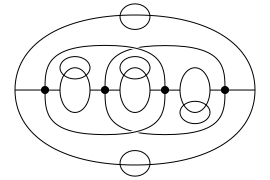
\includegraphics[width=2in]{pair-interference}
\end{center}
The pair of faces can make contact with each in several disconnected arcs, as shown above. Further, additional pair edges can share $F_1$ or $F_2$ with some other face. However, slicing $F_1$ can only separate $v_i$ and $v_j$ if the endpoints of the splitting arc link $v_i$ and $v_j$ on $F_1$. This can't happen if the splitting arc is part of a pair which share $F_1$ with some other face (as shown), as the interfaces of $F_1$ and other faces are all connected.

But if the splitting arc also shared $F_1$ and $F_2$, the corresponding pair variable $p_{k,l}$ is related to $p_{i,j}$ by a linking equation if and only if adding that arc would leave $v_i$ and $v_j$ on different faces. The linking equation implies that only one of the arcs indicated by $p_{i,j}$ and $p_{k,l}$ is present in the expansion; since we have assumed that $p_{i,j}$ is positive, no such $p_{k,l}$ can have already been inserted earlier in the expansion process. This concludes the case where the interface of $F_1$ and $F_2$ was disconnected.

\begin{center}
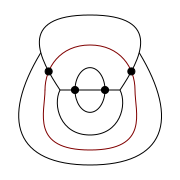
\includegraphics[width=2in]{connected-pair-interaction-case}
\end{center}

If the interface between $F_1$ and $F_2$ is connected, than either might have a disconnected interface with (at most one) other face, as shown above. This case is only cosmetically different-- again the key point is that the pair $v_i$, $v_j$ can link along the boundary of $F_1$ (or $F_2$) with a pair edge which also shares $F_1$ and $F_2$ while pairs involving a third face won't link the vertices we're interested in.

We last have only to observe that by the vertex degree equations, the final graph $G$ is a $4$-regular planar multigraph. Since we have only added edges along the way, $G$ is connected because $G_1$ was.
\end{proof}

We have reduced the problem to that of building and satisfying the vertex degree and linking equations. This problem is basically standard, and we use the usual branch-and-bound algorithm. We must define a canonical order on the variables (it doesn't matter how, but to be specific, in our implementation we sort the classes of variables in the order $l_i \prec d_{i,j} \prec c_{i,j} \prec p_{ij}$ and in dictionary order by the (sorted) pair $\{i,j\}$ within each class). Then we enumerate the possible assignments of $\{0,1\}$ to variables recursively, pruning the tree whenever a vertex degree or linking equation is violated. As usual, this is in theory possibly exponentially slow, but in practice efficient enough for small $n$.

We now consider the problem of dividing the results into embedded isomorphism classes. We first observe that we have already shown in Proposition~\ref{prop:reduce} two different reduced graphs $G_0$ and $G_0'$ cannot expand to the same $G$ since the embedded isomorphism type of the reduction $G_0$ is determined by the embedded isomorphism type of the expansion. However, it is possible for two different collections of expansion moves for the \emph{same} graph $G_0$ to produce isomorphic $G$ and $G'$ as in the picture below:
\begin{center}
\includegraphics[width=4in]{isomorphic-expansions}
\end{center}
Therefore, we must insert each expansion we generate from a solution to the vertex degree and linking constraints into a container which rejects the solution if an embedded isomorphic graph already exists in the container. Though very fast graph isomorphism checkers such as \nauty and \saucy might speed things up, the number of vertices here is very small and we get entirely acceptable performance simply by using a hashing scheme and then attempting to build isomorphisms by pruned search.

The overall workflow is then as follows:
\begin{center}
\includegraphics[width=4in]{workflow}
\end{center}

\section{Classifying knot types}

Our database of diagrams contains all diagrams of knots and links with $n$ crossings. Though very few of these are knot diagrams (the subject of this paper), there seems to be no obvious graph-theoretic way to avoid generating link diagrams. So our next move is to simply compute the number of components in each diagram and throw out the diagrams with more than one component. This gives us the following table of the number of diagrams we've found:

<data>

\begin{center}
Matt and Harrison write something about assigning crossings and orientations, and give data on expansions
\end{center}

\begin{center}
Matt and Harrison write something about their respective knot identification strategies and the verification that they match
\end{center}

\section{Results}

giant pictures, compared with tait's classification
our distributions
monogon and bigon fractions
degree of alternatingness
universal properties? comparison with distribution from ERPs, lattice walks, and petaluma.

An experiment to do: make a histogram of the number of diagrams which are all unknots, those that are mostly unknots, those that are partially unknots, and so forth.

I think this should partially explain the unknot fraction; the idea is that we should be able to count diagrams which can't possibly be knots (that is, stuff with only R1's) and see that while they eventually become exponentially scarce, they are (in this data) quite prevalent. Of course, it would be better if we also knew an upper bound on the total number of diagrams (maybe from Thistlethwaite's paper?), so that we could get an asymptotic bound on the decay rate.


\section{Future Directions}

transitions, unknotting number and so forth.

\bibliography{knotprobabilitypapers}


\end{document}
